
%%%%%%%%%%%%%%%%%%%%%%%%%%%%%%%%%%%%%%%
% IMPORTANT
\begin{spacing}{1} %THESE FOUR
\minitoc % LINES MUST APPEAR IN
\end{spacing} % EVERY
\thesisspacing % CHAPTER
% COPY THEM IN ANY NEW CHAPTER
%%%%%%%%%%%%%%%%%%%%%%%%%%%%%%%%%%%%%%%

% Define colors
\definecolor{agentic}{RGB}{46, 125, 50}
\definecolor{traditional}{RGB}{158, 158, 158}
\definecolor{llm}{RGB}{33, 150, 243}
\definecolor{collaborative}{RGB}{255, 152, 0}
\definecolor{limitation}{RGB}{244, 67, 54}

\chapter{Introduction to Recommender Systems}
\label{ch:intro}


\section{Formalism and Foundational Concepts}

Recommender systems are computational frameworks designed to predict user preferences for a set of items. Their function is to mitigate information overload by providing personalised suggestions from a vast item space. The economic and cultural impact of these systems is significant; major digital platforms attribute substantial revenue and user engagement to their recommendation engines \cite{linden2003amazon, schedl2018current}.

The fundamental task is to estimate a user's preference for an unobserved item given their historical interactions. The scale of this task presents a significant computational challenge. For instance, a service with $2 \times 10^8$ users and $1.5 \times 10^4$ items must evaluate a potential interaction space of $3 \times 10^{12}$ user-item pairs. To address this problem tractably, we establish a formal mathematical framework.

%TC:ignore
Let $\mathcal{U} = \{u_1, u_2, \ldots, u_m\}$ be the set of $m$ users and $\mathcal{I} = \{i_1, i_2, \ldots, i_n\}$ be the set of $n$ items. The core objective is to learn a prediction function $f$:
\begin{equation}
f: \mathcal{U} \times \mathcal{I} \rightarrow \mathbb{R}
\end{equation}
%TC:endignore
This function, $f(u, i)$, maps a user-item pair $(u, i)$ to a real-valued score $\hat{r}_{ui}$, which quantifies the predicted preference of user $u$ for item $i$.

These predictions are learned from observed historical data, typically represented as a sparse user-item interaction matrix, $\mathbf{R} \in \mathbb{R}^{m \times n}$. An entry $r_{ui}$ in this matrix represents the explicit rating (e.g., 1-5 stars) or implicit interaction (e.g., a click or purchase) between user $u$ and item $i$. Most entries in $\mathbf{R}$ are unknown.

The operational pipeline consists of two phases. During the \textbf{training} phase, the model learns the parameters of the prediction function $f$ by fitting to the set of observed interactions, $\mathcal{O} = \{(u, i, r_{ui}) \mid r_{ui} \text{ is known}\}$. In the subsequent \textbf{inference} phase, the trained function $f$ is used to compute preference scores $\hat{r}_{ui}$ for unobserved pairs. The items with the highest predicted scores for a given user are then recommended, typically as a top-$k$ list.

Several operational concepts are critical. The \textbf{cold-start problem} refers to scenarios with insufficient data for reliable prediction. It manifests in three forms: \textit{user cold-start} (a new user with no history), \textit{item cold-start} (a new item with no ratings), and \textit{system cold-start} (an entirely new platform). Conversely, \textbf{warm-start} scenarios, where users and items have rich interaction histories, are the ideal condition for most algorithms.

Two concepts of growing importance are \textit{explainability} and \textit{scrutability}. \textbf{Explainability} is the system's capacity to provide human-interpretable justifications for a recommendation. This moves beyond merely suggesting an item to providing rationale, such as "Recommended because you have positively rated other items in this genre." This transparency can foster user trust. \textbf{Scrutability} extends this by allowing users to inspect and actively manipulate the model's representation of their preferences. A scrutable system would enable a user to view their inferred taste profile and correct erroneous assumptions, thereby transforming the user from a passive recipient to an active participant in the recommendation process.


\subsection{A Historical Analysis}

The evolution of recommender systems is marked by distinct algorithmic paradigms.

\paragraph{Collaborative Filtering (1990s)} The field was established by the GroupLens project, which introduced user-based collaborative filtering (UBCF) \cite{resnick1994grouplens}. This approach relies on the principle that users with similar tastes will have similar future preferences. Similarity was formally calculated using metrics such as the Pearson correlation coefficient between user rating vectors:
%TC:ignore
\begin{equation}
\text{sim}(u,v) = \frac{\sum_{i \in \mathcal{I}_{uv}}(r_{ui} - \bar{r}_u)(r_{vi} - \bar{r}_v)}{\sqrt{\sum_{i \in \mathcal{I}_{uv}}(r_{ui} - \bar{r}_u)^2}\sqrt{\sum_{i \in \mathcal{I}_{uv}}(r_{vi} - \bar{r}_v)^2}}
\end{equation}
%TC:endignore
where $\mathcal{I}_{uv}$ is the set of items co-rated by users $u$ and $v$. Due to the scalability challenges of UBCF, item-based collaborative filtering (IBCF) was introduced, computing similarity between items instead of users \cite{sarwar2001item}. IBCF proved more computationally efficient and stable, as item-item relationships are often less dynamic than user-user relationships.

\paragraph{Matrix Factorization (2000s)} The Netflix Prize competition spurred a shift towards latent factor models, principally matrix factorization (MF) \cite{koren2009matrix}. MF techniques decompose the sparse interaction matrix $\mathbf{R}$ into low-dimensional user ($\mathbf{P} \in \mathbb{R}^{m \times f}$) and item ($\mathbf{Q} \in \mathbb{R}^{n \times f}$) latent factor matrices. A prediction is the inner product of a user's and an item's factor vectors, incorporating bias terms:
%TC:ignore
\begin{equation}
\hat{r}_{ui} = \mu + b_u + b_i + \mathbf{p}_u^T \mathbf{q}_i
\end{equation}
Here, $\mathbf{p}_u$ and $\mathbf{q}_i$ are the $f$-dimensional latent vectors for user $u$ and item $i$, and $\mu, b_u, b_i$ are the global, user, and item biases. The model is trained by minimising a regularised squared error objective over the observed ratings $\mathcal{O}$:
\begin{equation}
\min_{\mathbf{P},\mathbf{Q},\mathbf{b}} \sum_{(u,i) \in \mathcal{O}} (r_{ui} - \hat{r}_{ui})^2 + \lambda(\|\mathbf{p}_u\|^2 + \|\mathbf{q}_i\|^2 + b_u^2 + b_i^2)
\end{equation}
%TC:endignore
This formulation generalises well by learning dense representations that capture latent features underlying user preferences.

\paragraph{Deep Learning (2010s)} The advent of deep learning enabled the modelling of more complex, non-linear interactions. Early work like AutoRec used autoencoders to learn compact representations of interaction vectors \cite{sedhain2015autorec}. Neural Collaborative Filtering (NCF) generalised the MF inner product, replacing it with a multi-layer perceptron (MLP) to learn an arbitrary function between user and item latent vectors \cite{he2017neural}. Subsequently, attention mechanisms and Transformer architectures were adapted for sequential recommendation. Models like BERT4Rec use bidirectional self-attention to model user behaviour sequences, capturing complex dependencies within a user's interaction history \cite{sun2019bert4rec}.

%TC:ignore
\begin{figure}[h!]
    \centering
    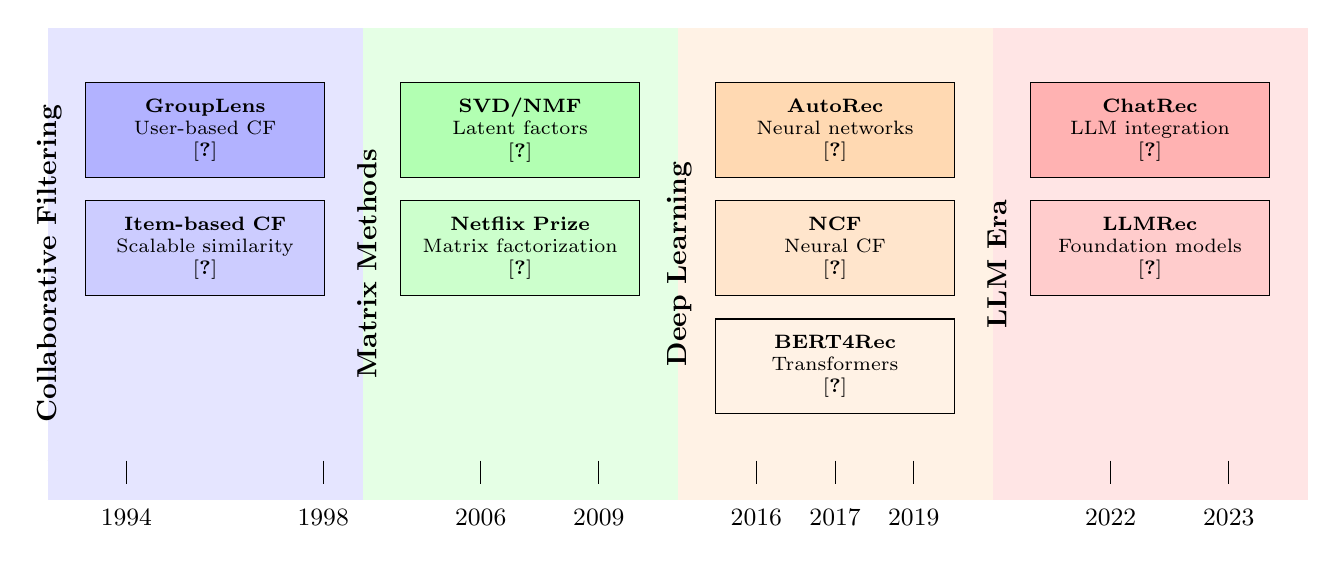
\begin{tikzpicture}[scale=1.0, every node/.style={transform shape}]
    % Timeline base
    \draw[thick, gray] (0,0) -- (16,0);
    
    % Era backgrounds - made taller and wider
    \fill[blue!10] (0,-0.5) rectangle (4,5.5);
    \fill[green!10] (4,-0.5) rectangle (8,5.5);
    \fill[orange!10] (8,-0.5) rectangle (12,5.5);
    \fill[red!10] (12,-0.5) rectangle (16,5.5);
    
    % Era labels - positioned better and larger font
    \node[rotate=90, font=\normalsize\bfseries, anchor=south] at (0.3,2.5) {Collaborative Filtering};
    \node[rotate=90, font=\normalsize\bfseries, anchor=south] at (4.3,2.5) {Matrix Methods};
    \node[rotate=90, font=\normalsize\bfseries, anchor=south] at (8.3,2.5) {Deep Learning};
    \node[rotate=90, font=\normalsize\bfseries, anchor=south] at (12.3,2.5) {LLM Era};
    
    % Timeline markers and events - better spacing
    \foreach \x/\year in {1/1994, 3.5/1998, 5.5/2006, 7/2009, 9/2016, 10/2017, 11/2019, 13.5/2022, 15/2023} {
        \draw (\x,0) -- (\x,-0.3);
        \node[below, font=\small] at (\x,-0.5) {\year};
    }
    
    % Key innovations with vertical alignment within each era
    % Collaborative Filtering Era (Blue)
    \node[draw, rectangle, fill=blue!30, minimum width=3cm, minimum height=1.2cm, text width=2.8cm, align=center, font=\scriptsize] at (2,4.2) {
        \textbf{GroupLens}\\
        User-based CF\\
        \cite{resnick1994grouplens}
    };
    
    \node[draw, rectangle, fill=blue!20, minimum width=3cm, minimum height=1.2cm, text width=2.8cm, align=center, font=\scriptsize] at (2,2.7) {
        \textbf{Item-based CF}\\
        Scalable similarity\\
        \cite{sarwar2001item}
    };
    
    % Matrix Methods Era (Green)
    \node[draw, rectangle, fill=green!30, minimum width=3cm, minimum height=1.2cm, text width=2.8cm, align=center, font=\scriptsize] at (6,4.2) {
        \textbf{SVD/NMF}\\
        Latent factors\\
        \cite{lee1999learning}
    };
    
    \node[draw, rectangle, fill=green!20, minimum width=3cm, minimum height=1.2cm, text width=2.8cm, align=center, font=\scriptsize] at (6,2.7) {
        \textbf{Netflix Prize}\\
        Matrix factorization\\
        \cite{koren2009matrix}
    };
    
    % Deep Learning Era (Orange)
    \node[draw, rectangle, fill=orange!30, minimum width=3cm, minimum height=1.2cm, text width=2.8cm, align=center, font=\scriptsize] at (10,4.2) {
        \textbf{AutoRec}\\
        Neural networks\\
        \cite{sedhain2015autorec}
    };
    
    \node[draw, rectangle, fill=orange!20, minimum width=3cm, minimum height=1.2cm, text width=2.8cm, align=center, font=\scriptsize] at (10,2.7) {
        \textbf{NCF}\\
        Neural CF\\
        \cite{he2017neural}
    };
    
    \node[draw, rectangle, fill=orange!10, minimum width=3cm, minimum height=1.2cm, text width=2.8cm, align=center, font=\scriptsize] at (10,1.2) {
        \textbf{BERT4Rec}\\
        Transformers\\
        \cite{sun2019bert4rec}
    };
    
    % LLM Era (Red)
    \node[draw, rectangle, fill=red!30, minimum width=3cm, minimum height=1.2cm, text width=2.8cm, align=center, font=\scriptsize] at (14,4.2) {
        \textbf{ChatRec}\\
        LLM integration\\
        \cite{gao2023chat}
    };
    
    \node[draw, rectangle, fill=red!20, minimum width=3cm, minimum height=1.2cm, text width=2.8cm, align=center, font=\scriptsize] at (14,2.7) {
        \textbf{LLMRec}\\
        Foundation models\\
        \cite{bao2023tallrec}
    };
    
    \end{tikzpicture}
    \caption{The evolution of recommender systems, illustrating the progression of algorithmic paradigms from early collaborative filtering to contemporary Large Language Model-based approaches.}
    \label{fig:recsys_timeline}
\end{figure}
%TC:endignore

\subsection{Key Research Challenges in the Field}

This historical progression reveals persistent challenges that define the research frontier. A critical insight, articulated by Koren, is that the performance of a recommender system is determined more by \textbf{the quality and expressiveness of its input features} than by the sophistication of its learning algorithm \cite{koren2009matrix}. While neural architectures have grown more powerful, empirical evidence indicates diminishing returns, where substantial computational costs yield only marginal improvements. This positions \textbf{feature engineering}---the process of creating expressive inputs---as the primary bottleneck. Consequently, advancing the quality and acquisition of features, rather than merely increasing model complexity, has become the frontier for meaningful progress. This focus directly informs the principal challenges facing the field.

The most fundamental of these is \textbf{data sparsity and the cold-start problem}, which is, in essence, a problem of feature absence. An effective system must be capable of generating high-quality recommendations from minimal interaction data. This necessitates transfer learning or meta-learning mechanisms to bootstrap recommendations for new users and items.

Finally, research is ongoing in the field on improving \textbf{explainability and scrutability}. If feature quality is paramount, then a system must be able to articulate which features drove a given recommendation. Moving beyond predictive accuracy, the goal is to create systems that are transparent and user-controllable. Research in this area focuses on generating explanations that are both faithful to the model's internal logic and comprehensible to a non-expert user. Achieving full scrutability---allowing users to inspect and correct the model's preference profile---remains a significant challenge in Human-Computer Interaction (HCI) and Machine Learning.



\section{Large Language Models (might) be all we need}

To address these fundamental issues, LLMs are a great candidate. They can be used to converse directly with the user, and provide explainable recommendations, provide scrutability, and be used for upstream tasks such as Feature Engineering.
\begin{figure}[h!]
\centering
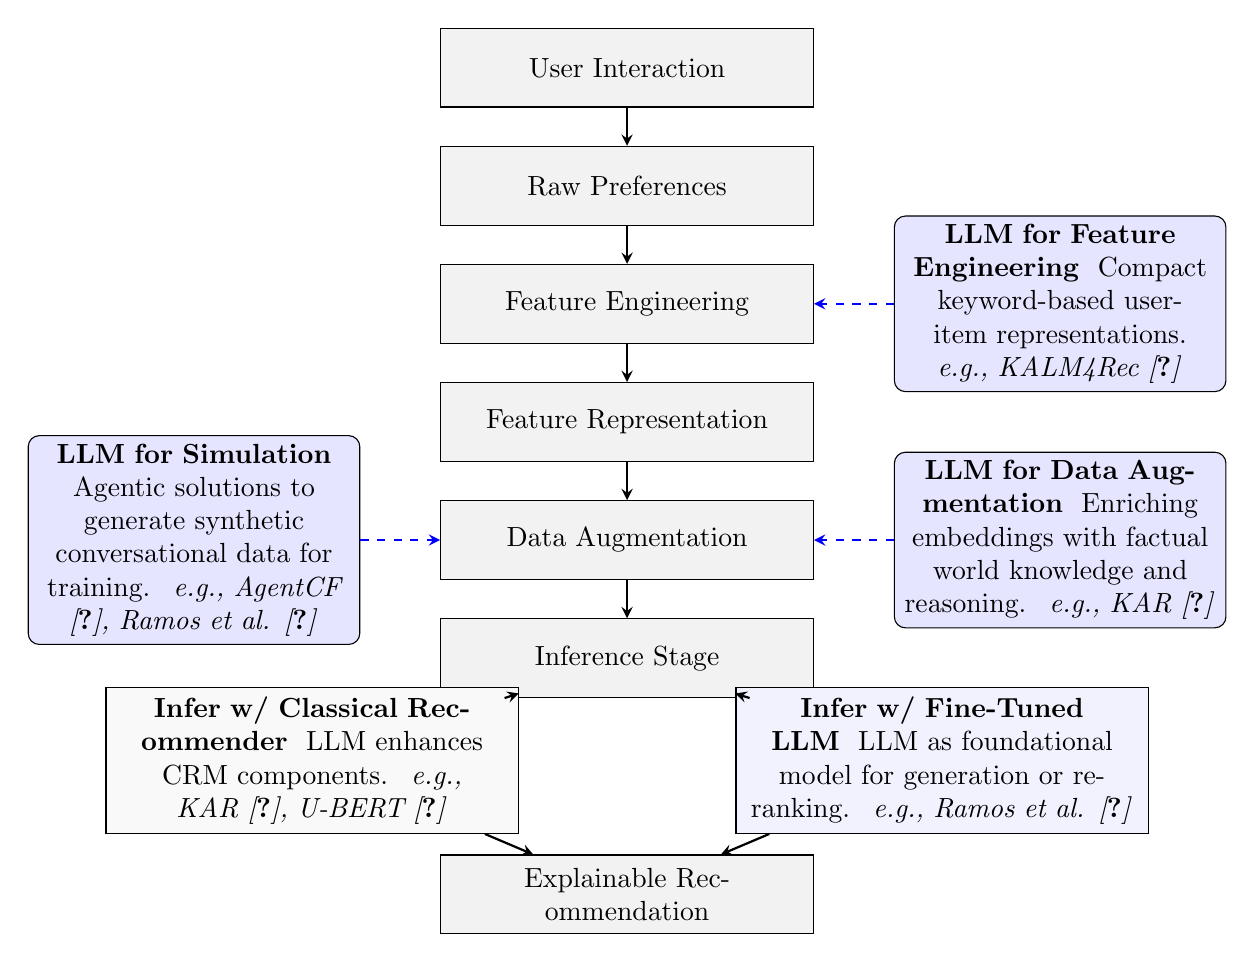
\begin{tikzpicture}[
node distance=1.5cm,
pipeline/.style={rectangle, draw, fill=gray!10, text centered, minimum height=1cm, text width=4.5cm},
llm_intervention/.style={rectangle, draw, fill=blue!10, rounded corners, text centered, text width=4cm, inner sep=3pt},
arrow/.style={->, >=stealth, thick}
]

% Define nodes
\node (interaction) [pipeline] {User Interaction};
\node (raw_prefs) [pipeline, below of=interaction] {Raw Preferences};
\node (feat_eng) [pipeline, below of=raw_prefs] {Feature Engineering};
\node (feat_rep) [pipeline, below of=feat_eng] {Feature Representation};
\node (data_aug) [pipeline, below of=feat_rep] {Data Augmentation};
\node (inference) [pipeline, below of=data_aug] {Inference Stage};
\node (explain) [pipeline, below of=inference, yshift=-1.5cm] {Explainable Recommendation};

% LLM Intervention Nodes
\node (llm_feat_eng) [llm_intervention, right of=feat_eng, xshift=4cm] {\textbf{LLM for Feature Engineering} \ Compact keyword-based user-item representations. \ \textit{e.g., KALM4Rec \cite{kieu2024keyword}}};
\node (llm_data_aug) [llm_intervention, right of=data_aug, xshift=4cm] {\textbf{LLM for Data Augmentation} \ Enriching embeddings with factual world knowledge and reasoning. \ \textit{e.g., KAR \cite{xi2023towards}}};
\node (llm_sim) [llm_intervention, left of=data_aug, xshift=-4cm] {\textbf{LLM for Simulation} \ Agentic solutions to generate synthetic conversational data for training. \ \textit{e.g., AgentCF \cite{zhang2023agentcf}, Ramos et al. \cite{ramos2024transparent}}};

% Inference Split
\node (crm) [pipeline, below of=inference, xshift=-4cm, yshift=0.2cm, fill=gray!5, text width=5cm] {\textbf{Infer w/ Classical Recommender} \ LLM enhances CRM components. \ \textit{e.g., KAR \cite{xi2023towards}, U-BERT \cite{qiu2021u}}};
\node (llm_inf) [pipeline, below of=inference, xshift=4cm, yshift=0.2cm, fill=blue!5, text width=5cm] {\textbf{Infer w/ Fine-Tuned LLM} \ LLM as foundational model for generation or re-ranking. \ \textit{e.g., Ramos et al. \cite{ramos2024transparent}}};

% Arrows
\draw [arrow] (interaction) -- (raw_prefs);
\draw [arrow] (raw_prefs) -- (feat_eng);
\draw [arrow] (feat_eng) -- (feat_rep);
\draw [arrow] (feat_rep) -- (data_aug);
\draw [arrow] (data_aug) -- (inference);
\draw [arrow] (inference) -- (crm);
\draw [arrow] (inference) -- (llm_inf);
\draw [arrow] (crm) -- (explain);
\draw [arrow] (llm_inf) -- (explain);

% LLM Intervention Arrows
\draw [arrow, dashed, blue] (llm_feat_eng.west) -- (feat_eng.east);
\draw [arrow, dashed, blue] (llm_data_aug.west) -- (data_aug.east);
\draw [arrow, dashed, blue] (llm_sim.east) -- (data_aug.west);

% Feedback Loop


\end{tikzpicture}
\caption{The recommender system pipeline illustrating specific stages where LLMs are applied. LLMs can enhance traditional steps like \textbf{Feature Engineering} by creating structured, keyword-based representations from raw data. They are also used for \textbf{Data Augmentation}, where they enrich user and item embeddings with external world knowledge and reasoning capabilities. Separately, LLMs are used for \textbf{Simulation}, where autonomous agents generate synthetic conversational data, a crucial step for training models when real-world datasets are unavailable. Finally, LLMs can replace or supplement the \textbf{Inference} stage to produce explainable outputs.}
\label{fig:llm_pipeline}
\end{figure}

While direct LLM-based recommendation generation demonstrates impressive zero-shot capabilities \cite{dai2023uncovering}, we believe pursuing feature engineering with LLMs presents a more promising and sustainable approach for several empirically-supported reasons. Computational efficiency analyses reveal that direct LLM inference for recommendation tasks incurs prohibitive costs at scale, with Zhao et al. \cite{zhao2023rellm} demonstrating that LLM-based ranking requires 100x more computational resources than traditional collaborative filtering approaches when serving millions of users. Kang et al. \cite{kang2023llms} further show that while LLMs exhibit reasonable zero-shot recommendation performance, they consistently underperform fine-tuned collaborative filtering models on standard benchmarks, particularly for users with rich interaction histories where collaborative signals provide superior preference modeling. Feature engineering with LLMs enables hybrid architectures that capture the best of both paradigms: Li et al. \cite{li2023text} demonstrate that LLM-generated semantic features combined with collaborative filtering achieve superior performance compared to either approach alone, while maintaining computational tractability through offline feature generation. The interpretability advantages are equally compelling, as Bao et al. \cite{bao2023tallrec} show that LLM-generated features provide human-interpretable semantic dimensions that enable systematic analysis and improvement, contrasting with the black-box nature of end-to-end LLM recommendations. Most critically, Hua et al. \cite{hua2023up5} empirically demonstrate that hybrid approaches synthesizing LLM-derived semantic understanding with collaborative filtering signals consistently outperform pure LLM-based systems across multiple domains, suggesting that the integration of semantic and behavioral signals through feature engineering represents a more robust foundation for next-generation recommender systems than direct LLM-based generation.

\subsection{Enter Automated Feature Engineering...}

Feature engineering transforms raw data into predictive signals for ML models. In recommender systems, this is complicated by interaction matrix sparsity (typically >99\% sparse), cold-start problems, and non-stationary user preferences \cite{schein2002cold}.

Traditional approaches require domain expertise and iterative manual feature construction, creating development bottlenecks. Automated Feature Engineering (AutoFE) addresses this through systematic feature generation and evaluation without human intervention.

Deep Feature Synthesis (DFS) \cite{kanter2015deep} provides the foundational framework, composing primitive operations (aggregation, transformation, selection) to construct complex features recursively. Implemented in libraries like \texttt{featuretools}\footnote{https://github.com/alteryx/featuretools}, DFS explores feature transformation spaces systematically by applying operations at increasing depths.

However, combinatorial AutoFE suffers from exponential feature space explosion—generating \(10^4 -10^5\) candidates with low signal-to-noise ratios. These systems lack semantic awareness and domain knowledge, producing syntactically valid but often meaningless features. The resulting computational overhead for downstream feature selection frequently exceeds generation costs, while failing to identify domain-relevant feature interactions.


\subsubsection{From Combinatorial Automation to LLMs}

CAAFE \cite{hollmann2023caafe} pioneered using GPT-3.5 to iteratively generate and refine Python code for feature transformations, achieving ROC AUC improvements from 0.798 to 0.822 across datasets, while FEBP \cite{zou2025febp} enhanced this approach through canonical Reverse Polish Notation and temperature-controlled generation. \\

However, these single-agent systems suffer from fundamental limitations including lack of strategic reasoning, inability to leverage diverse analytical perspectives, and unsystematic exploration of the feature space.\\

The constraints of single-agent approaches have motivated research into multi-agent systems where specialized AI agents collaborate on complex tasks. Frameworks like AutoGen \cite{wu2023autogen} enable structured collaboration through conversational agents with distinct roles, while MetaGPT \cite{hong2023metagpt} demonstrates how role specialization (product manager, architect, engineer) enhances collaborative problem-solving in software development contexts. These systems illustrate the potential of multi-agent coordination theory \cite{tran2025multiagent}, which identifies key collaboration dimensions including actor roles, interaction types, organizational structures, and coordination protocols. However, existing multi-agent frameworks remain general-purpose tools lacking the domain-specific reasoning patterns, evaluation mechanisms, and optimization strategies required for effective feature engineering in recommender systems.

Current approaches exhibit critical gaps that prevent realization of truly intelligent automated feature engineering. Existing systems apply domain-agnostic reasoning without incorporating recommender-specific patterns like collaborative filtering principles or temporal user behavior dynamics. They rely on ad-hoc feature generation rather than systematic exploration of feature categories (temporal, contextual, collaborative, content-based) through specialized analytical perspectives. Most critically, they treat feature evaluation as disconnected post-processing rather than integrating it through bilevel optimization frameworks that simultaneously optimize feature discovery strategies and implementation quality. Additionally, current systems lack collaborative validation mechanisms where multiple agents critique and refine proposals, missing the quality assurance benefits of human data science team collaboration.


These limitations motivate the development of specialized agentic approaches that combine domain-aware feature engineering with collaborative multi-agent intelligence and rigorous optimization frameworks. 



\section{Research Questions and Contributions}

This thesis addresses the critical gap in automated feature engineering for recommender systems through the development of collaborative multi-agent systems. Cold-start recommendation problems—where new users or items lack sufficient interaction history—represent particularly challenging scenarios that require sophisticated feature engineering to capture meaningful patterns from limited data. The research is guided by four principal questions that examine both the technical foundations and practical applications of agentic feature engineering.

\textbf{RQ1:} - How can multi-agent collaborative systems be architected to perform end-to-end feature engineering for cold-start recommendation problems, and what agent coordination mechanisms enable effective optimization of both feature discovery and hyperparameter tuning?\\
\textbf{RQ2:} - To what extent can the integration of agent-generated parameterized features with Bayesian optimization improve feature quality compared to traditional automated feature engineering approaches?\\
\textbf{RQ3:} - How effectively can agentic feature engineering systems employ meta-learning to self-improve their feature discovery strategies across different datasets and recommendation contexts?\\
\textbf{RQ4:} - What are the performance gains of agentic feature engineering in cold-start recommendation scenarios, and how do these compare to existing automated and manual feature engineering approaches?\\

To address these research questions, this thesis introduces AGENTIC (Autonomous Group Engineering for Next-generation Tabular Intelligence and Collaborative discovery), a novel end-to-end framework for feature engineering in cold-start recommendation systems. The system employs collaborative multi-agent teams to optimize clustering-based user assignment through Bayesian questioning, with the feature engineering component serving as the foundation for this broader recommendation pipeline. The key contributions of this research are threefold:

\textbf{Contribution 1: An end-to-end agentic framework} - We present the first comprehensive framework that integrates multi-agent feature engineering with cold-start recommendation systems. While this thesis focuses on the feature engineering component (which has been open-sourced), the complete system represents a fully testable framework for addressing cold-start scenarios through collaborative AI optimization of user clustering and assignment via Bayesian questioning mechanisms.

\textbf{Contribution 2: An open-source parameterised feature engineering with Bayesian Optimization} - We introduce a novel approach where features are defined as agent-generated functions with explicit hyperparameters, subsequently optimized through Bayesian optimization for fine-grained parameter estimation. This dual-level optimization strategy—combining agent creativity with systematic parameter tuning—represents a significant advancement over existing automated feature engineering approaches that typically generate fixed-form features.

\textbf{Contribution 3: Self-Improving Agentic Workflows} - We demonstrate one of the first implementations of agentic workflows capable of meta-learning and self-improvement in feature engineering contexts. The system learns from its feature engineering experiences across datasets, adapting its discovery strategies and improving performance over time through accumulated knowledge and refined coordination mechanisms.

These contributions establish agentic feature engineering as a new paradigm that combines the creative reasoning capabilities of large language models with systematic optimization principles and collaborative intelligence. The framework addresses fundamental limitations of existing automated approaches while providing a foundation for advancing both feature engineering methodologies and cold-start recommendation systems.
